%%% Třetí kapitola

\chapter{Testování algoritmu na datech}

V této sekci představíme výsledky implementace výpočtu Jonesova polynomu. Změříme délku běhu algoritmu a jeho variant na malých uzlech, náhodých uzlech a lincích a na speciálních typech uzlů.

Varianty

\section{Malé tabulkové uzly}

\begin{figure}[p]\centering
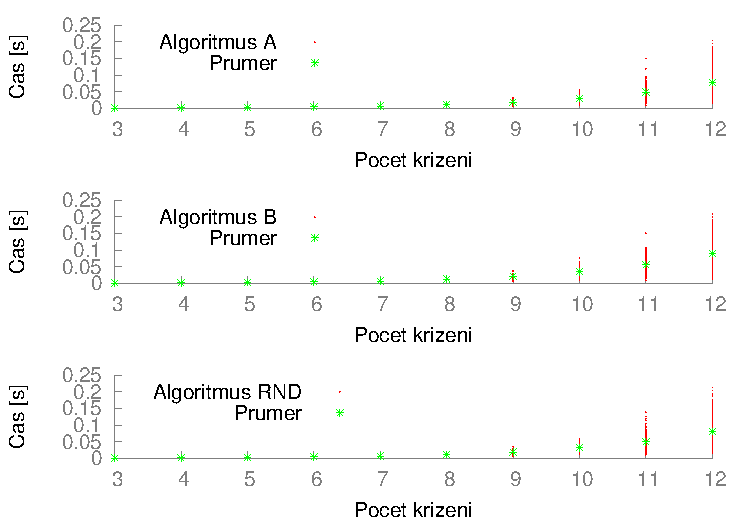
\includegraphics{../img/multiTable}
\caption{Graf dob běhu algoritmů na tabulkových uzlech do 12 křížení s vyznačenými průměry.}
\label{obr03:multiTable}
\end{figure}

Algoritmy jsme vyzkoušely na všech uzlech, které mají projekci s maximálně dvanácti kříženími. PD notace uzlů byla získána z databáze KnotInfo. 
U všech tří algoritmů byl už u malých uzlů znatelný exponenciální růst doby běhu (viz Obrázek~\ref{obr03:multiTable}).
 

Ze srovnání průměrných dob běhu plyne, že nejlepší čas dosahuje algoritmus A, těsně následuje algoritmus RND a nejpomalejší je algoritmus B (viz Obrázek~\ref{obr03:srovTable}). Podobné výsledky se budou objevovat i nadále.
	
\begin{figure}[p]\centering
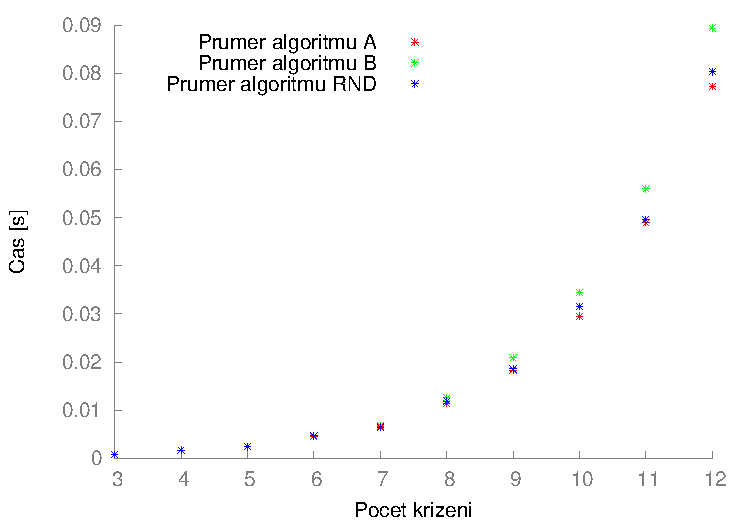
\includegraphics{../img/srovTable}
\caption{Graf průměrných časů algoritmů na tabulkových uzlech do 12 křížení.}
\label{obr03:srovTable}
\end{figure}


\section{Náhodné uzly a linky}

\subsection{Generování náhodných linků a uzlů}
Náhodné linky budeme generovat pomocí rovinných grafů, neboť mezi linky a rovinnými grafy existuje vzájemně jednoznačná korespondence, zdroj?. (Jedná se o jinou korespondenci,  než tu mezi linky a rovinnými grafy s vrcholu stupně čtyři popsanou v sekci **).

\subsubsection{Převod rovinného grafu na link}
Rovinný graf z $n$ hranami odpovídá linku s $n$ kříženími. Každé hraně přířadíme náhodně kladné, či záporné znamení a umístíme na ni křížení příslušného typu. Úseky mezi kříženími jsou tím již jednoznačně určené: musí spojovat křížení mezi nejbližšími hranami tak, aby nevznikla žádná další křížení.

OBRÁZEK, KRESLENÝ RUKOU

\subsubsection{Generování náhodných rovinných grafů}
Graf s $n$ hranami získáme následujícím způsobem. Vygenerujeme vhodný počet náhodných bodů v rovině a nalezeneme jejich triangulaci, tj. spojíme body hranami tak, aby byl polygon tvořící konvexní obal bodů rozdělen na trojúhelníky.

\begin{figure}[h]  
\centering 
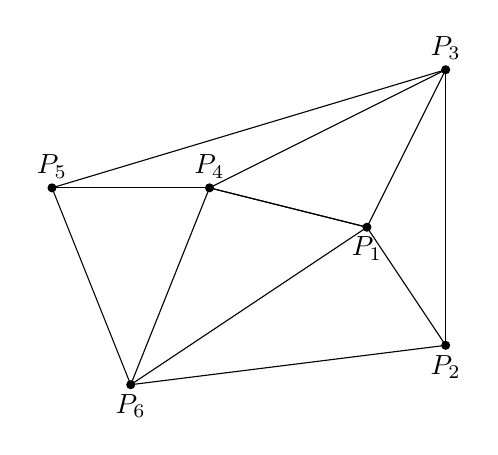
\begin{tikzpicture}
\draw[fill] (1,1) circle [radius=0.05];
\node [below] at (1,1) {$P_1$};

\draw[fill] (2,-1/2) circle [radius=0.05];
\node [below] at (2,-1/2) {$P_2$};

\draw[fill] (2,3) circle [radius=0.05];
\node [above] at (2,3) {$P_3$};

\draw[fill] (-1,3/2) circle [radius=0.05];
\node [above] at (-1,3/2) {$P_4$};

\draw[fill] (-3,3/2) circle [radius=0.05];
\node [above] at (-3,3/2) {$P_5$};

\draw[fill] (-2,-1) circle [radius=0.05];
\node [below] at (-2,-1) {$P_6$};

\draw (-3,3/2) -- (2,3);
\draw (-3,3/2) -- (-1,3/2);
\draw (-3,3/2) -- (-2,-1);
\draw (-1,3/2)  -- (2,3) ;
\draw (-1,3/2)  -- (-2,-1) ;
\draw (-1,3/2)  -- (1,1) ;
\draw (-1,3/2)  -- (1,1) ;
\draw (2,3)   -- (1,1) ;
\draw (-2,-1) -- (1,1) ;
\draw (-2,-1) -- (2,-1/2);
\draw  (1,1)  -- (2,-1/2);
\draw  (2,3)-- (2,-1/2);
\end{tikzpicture}
\caption{Triangulace šesti bodů}
\end{figure}  

Získali jsme tak rovinný graf s původními body jako vrcholy. Pokud je počet hran menší než $n$, provedeme triangulaci znovu s větším počtem bodů. Pokud je počet hran větší než $n$, odstraníme potřebný počet náhodně zvolených hran.

\subsubsection{Implementace}

Triangulace bodů je snadno implementovatelný geometrický problém. \\ Se získaným rovinným grafem pracujeme jako s množinou vrcholů a k nim příslušným hranám seřazeným v pořadí, jak k danému vrcholu přiléhají. Z této struktury je již možné získat PD notaci příslušného linku.


V PD notaci lze procházkou po vláknu snadno poznat, jestli je vygenerovaný link uzlem. Také jsme v PD notaci jednoduchou operací schopni uzel změnit na alternující, tedy takový, v němž se střídají křížení vedená zespodu a zvrchu.

Jsme tedy schopni nagenerovat uzly, alternující uzly a linky libovolné velikosti.

Takto generované uzly jsou také poměrně \uv{zamotané}, tedy rozmotávací krok algoritmu neodstraní příliš mnoho křížení.

\subsection{Test}

\begin{figure}[p]\centering
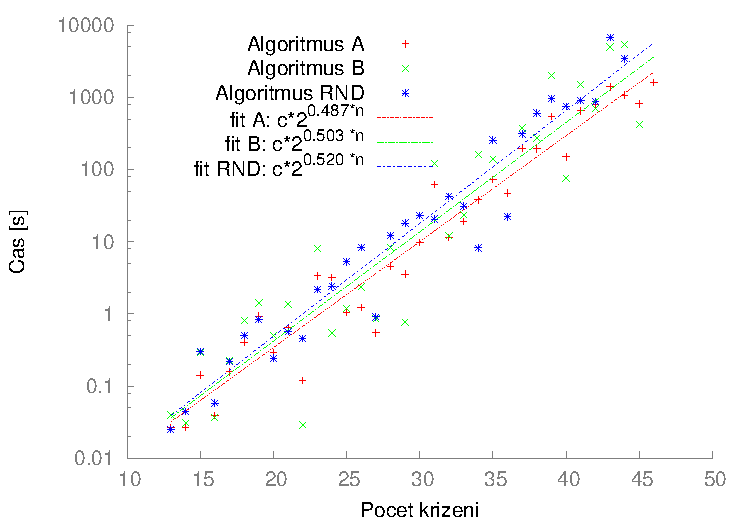
\includegraphics{../img/knotsFIT}
\caption{Graf dob běhu algoritmů náhodných uzlech proložené křivkami, logaritmická škála.}
\label{obr03:knotSrov}
\end{figure}

\begin{figure}[p]\centering
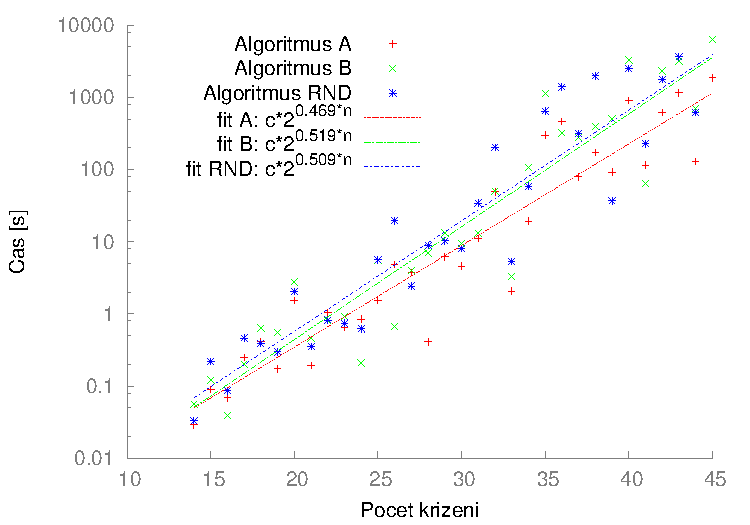
\includegraphics{../img/alt_knotsFIT}
\caption{Graf dob běhu algoritmů na náhodných alternujících uzlech proložené křivkami, logaritmická škála.}
\label{obr03:altSrov}
\end{figure}

\begin{figure}[p]\centering
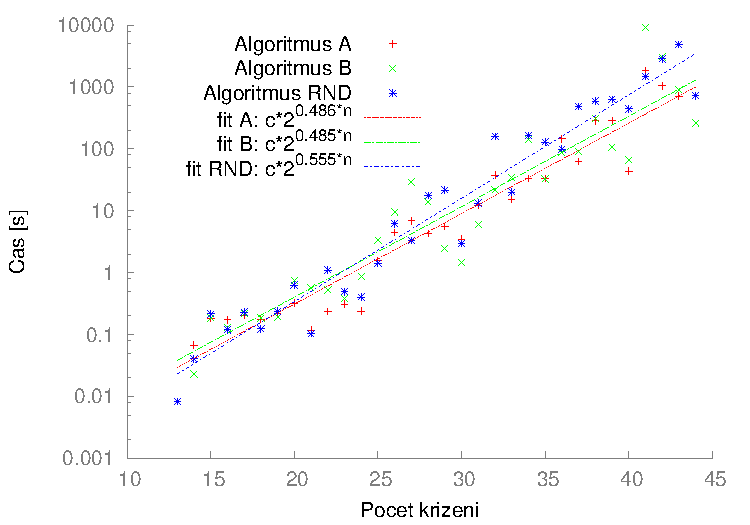
\includegraphics{../img/linksFIT}
\caption{Graf dob běhu algoritmů na náhodných lincích proložené křivkami, logaritmická škála.}
\label{obr03:linkSrov}
\end{figure}

Rychlost algoritmů jsme tedy otestovali na uzlech (Obrázek~\ref{obr03:knotSrov}) , alternujících uzlech (Obrázek~\ref{obr03:altSrov}) a lincích (Obrázek~\ref{obr03:linkSrov}) s počtem křížení do 46. 

Podle výsledků není znatelný rozdíl mezi dobou výpočtu na uzlech, alternujících uzlech či lincích. Ani jednotlivé algoritmy se od sebe výrazně neliší, nejrychleji ale Jonesův polynom vždy počítá algoritmus A. Jeho průměrná časová složitost je podle naměřených dat menší než $\mathcal{O}(2^{0,5n})$. 

Na uzlech a alternujících uzlech běží algoritmy B i RND podobnou dobu, liší se na ovšem na lincích. Zde se algoritmus B vyrovná algoritmu A, ale algoritmus RND zaostává. Náhodná volba křížení k rozpojení pravděpodobně způsobí rozpadnutí na větší počet stále zamotaných linků.

Odhad průměrné časové složitosti
Chyby maximálně pět procent.

\begin{table}[b!]

\centering
%%% Tabulka používá následující balíčky:
%%%   - booktabs (\toprule, \midrule, \bottomrule)
%%%   - dcolumn (typ sloupce D: vycentrovaná čísla zarovnaná na
%%%     desetinnou čárku
%%%     Všimněte si, že ve zdrojovém kódu jsou desetinné tečky, ale
%%%     tisknou se čárky.
%%% Dále používáme příkazy \pulrad a \mc definované v makra.tex

\begin{tabular}{l@{\hspace{1.5cm}}D{.}{,}{3}D{.}{,}{1.3}D{.}{,}{2.4}} 
\toprule
 & \mc{} & \mc{} & \mc{} \\
\mc{} & \mc{\pulrad{\textbf{A}}} & \mc{\pulrad{\textbf{B}}} &
\mc{\pulrad{\textbf{RND}}} \\
\midrule
Uzly     & 0.487 & 0.503& 0.520 \\
Alternující uzly & 0.469 & 0.519 & 0.509 \\
Linky   & 0.486 & 0.485 &  0.555\\
\bottomrule
\end{tabular}

\caption{Odhady parametru $k$ průměrné časové složitosti $\mathcal{O}(2^{kn})$ jednotlivých algoritmů.}\label{tab03:algo}

\end{table}


\section{Torusové uzly}
Rychlost algoritmů jsme vyzkoušeli na 36 nejmenších torusových uzlech. Jejich PD notaci jsme získali z databáze knot atlas.

TO není torusový uzel!! Ale znamená to, že z toho dokážu vyrobit link? To by bylo fajn. Zmenším. A dám vedle toho. Pěkné to bude.

\begin{figure}[p]\centering
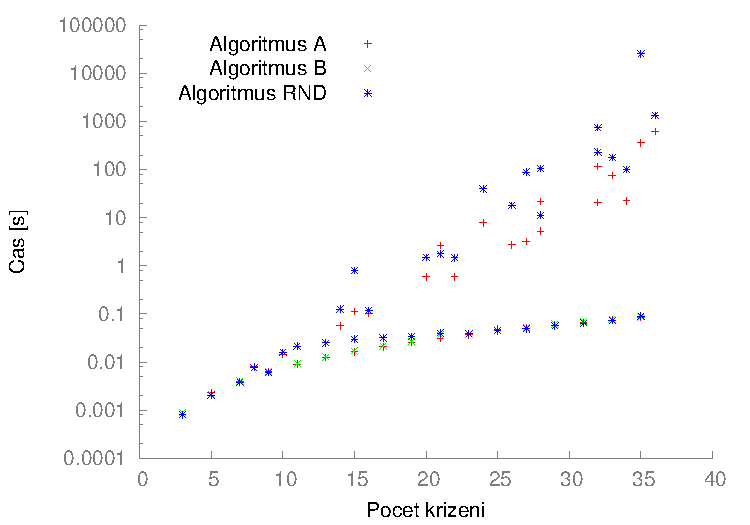
\includegraphics{../img/torusSrov}
\caption{Graf dob běhu algoritmů na 36 torusových uzlech, logaritmická škála.}
\label{obr03:torusSrov}
\end{figure}

Na grafu dob běhu algoritmů lze rozlišit dva shluky bodů (viz Obrázek~\ref{obr03:torusSrov}). Spodní shluk odpovídá torusovým uzlům ($2k+1$, 2), tedy těm, které se obmotají dvakrát podél osy rotace torusu a jejich diagram má tvar dvou zakroucených vláken s $2k+1$ kříženími.

\begin{figure}[h]\centering
\begin{tikzpicture}[use Hobby shortcut]
\begin{knot}[
  consider self intersections=true,
%  draft mode=crossings,
  flip crossing/.list={2,4,6} 
]
\strand ([closed]90:2) foreach \k in {1,...,7} { .. (90-360/7+\k*720/7:1.5) .. (90+\k*720/7:2) } (90:2);
\end{knot}
\end{tikzpicture}
\caption{Torusový uzel (7,2).}
\label{obr03:torus7}
\end{figure}

\begin{figure}[p]\centering
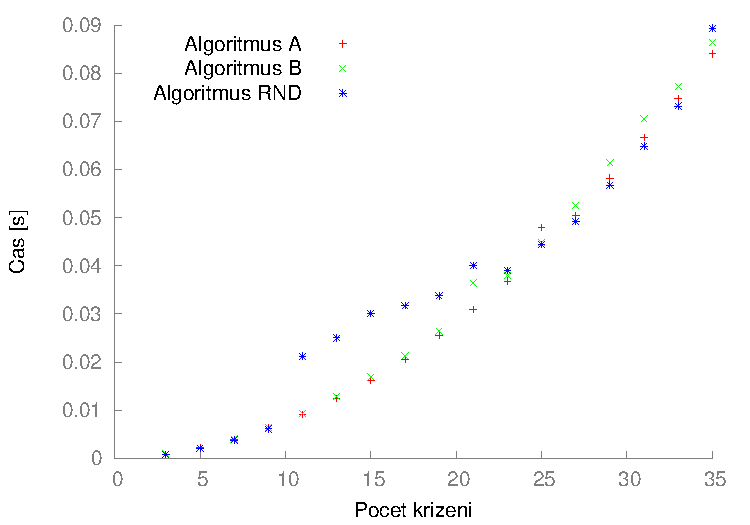
\includegraphics{../img/torus2}
\caption{Doby běhu algoritmů na torusových uzlech (3,2) až (35,2).}
\label{obr03:torus2}
\end{figure}

Všechny stěny tohoto uzlu jsou ohraničené pouze dvěma hranami. Rozpojením libovolného křížení jedním směrem vznikne torusový link ($2k$, 2), druhým směrem triviální uzel, který lze rozmotat někalika prvními Reidemeistrovými pohyby. Z linku zase rozpojením libovolného křížení vznikne uzel ($2k-1$, 2). Rozpojení a rozmotávání má lineární časovou složitost, celkově tedy všechny tři algoritmy spočítají Jonesův polynom tohoto typu torusových uzlů v kvadratickém čase (viz Obrázek~\ref{obr03:torus2}).

\begin{figure}[p]\centering
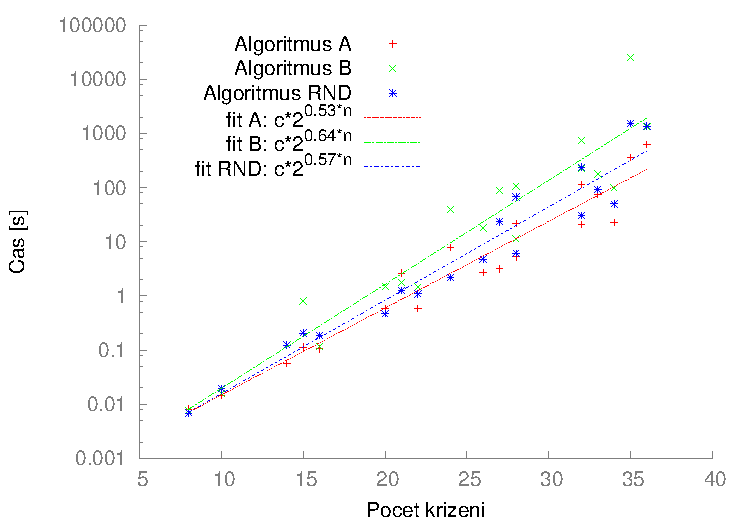
\includegraphics{../img/torusNe2FIT}
\caption{Doby běhu algoritmů na malých torusových uzlech ($p$, $q\neq 2$) proložené křivkami, logaritmická škála.}
\label{obr03:torusFIT}
\end{figure}

Na torusových uzlech tvaru ($p$, $q$), kde $q\neq 2$ již doba běhu algoritmu roste exponenciálně. Nejrychlejší je algoritmus A, příslušná  exponenciála je tvaru $2^{53n}$ (viz Obrázek~\ref{obr03:torusFIT}).

Nezapomenou dělat závěry a shrnovat.

